%%%%%%%%%%%%%%%%%%%%% chapter.tex %%%%%%%%%%%%%%%%%%%%%%%%%%%%%%%%%
%
% sample chapter
%
% Use this file as a template for your own input.
%
%%%%%%%%%%%%%%%%%%%%%%%% Springer-Verlag %%%%%%%%%%%%%%%%%%%%%%%%%%


\chapstarthook{The content of this chapter corresponds with the
following publication: \textbf{J.A. Aguilar, I. Garrig{\'o}s, J.-N. Maz{\'o}n. Impact Analysis of Goal-Oriented Requirements in Web Engineering. The 11th  International Conference on Computational Science and Its Applications (ICCSA 2011), June 20-23, 2011, Santander, Spain. Part V, Lecture Notes in Computer Science, Vol. 6786, pp. 421-436, 2011.}}


\chapter{Impact Analysis of Goal-Oriented Requirements in Web Engineering}
\label{c5} % Always give a unique label
% use \chaptermark{}
% to alter or adjust the chapter heading in the running head

The previous chapters begin by defining multidimensional models at
the conceptual level. However successful data warehouse design needs
to be based upon a requirement analysis phase if it is to adequately
represent the information needs of decision makers. Moreover, since
the data warehouse integrates the information provided by data
sources, it is also crucial to take these sources into account
throughout the development process in order to obtain a consistent
reconciliation of data sources and information needs. In this
chapter, a requirement analysis approach for multidimensional
modeling of data warehouses and the corresponding reconciliation
process is developed. The content of this chapter corresponds with
the part of the approach shaded in the figure below.


%\begin{figure}[h!]
%  \begin{center}
%    \includegraphics[width=0.7\textwidth]{img/chapters/chapter5}
%  \end{center}
%  %\caption{} \label{}
%\end{figure}


The content of this chapter corresponds with a paper published in
the \emph{Data \& Knowledge Engineering (DKE)} journal. This reaches
a world-wide audience of researchers, designers, managers and users.
The major aim of the journal is to identify, investigate and analyze
the underlying principles in the design and effective use of
database and knowledgebase systems. This journal publishes original
research results, technical advances and news items concerning data
engineering, knowledge engineering, and the interface of these two
fields. It should also be mentioned that this journal had an
\emph{impact factor} of \emph{1.144} in 2007, according to the
\emph{Thomson's Science Citation Index (SCI)}
(\url{http://www.isiwebofknowledge.com/}).

Finally, it is worth mentioning that this paper has been ranked by
\emph{ScienceDirect} (\url{http://www.sciencedirect.com/}) as one of
the \emph{25 hottest articles} published in DKE during last quarter
of 2007 (\url{http://top25.sciencedirect.com}).
%(\url{http://top25.sciencedirect.com/subject/engineering/12/journal/data-knowledge-engineering/0169023X/archive/14/})


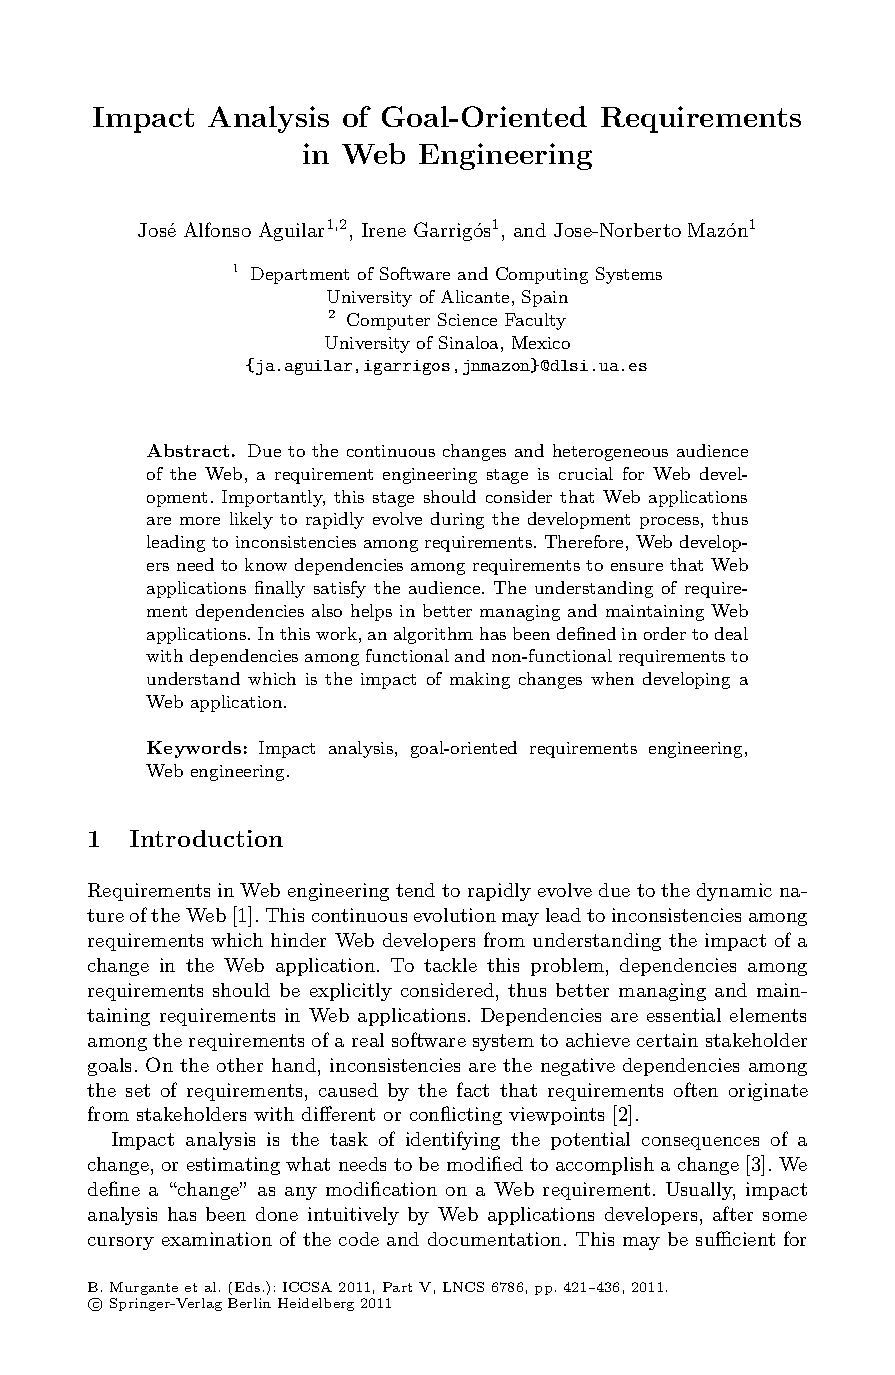
\includepdf[openright=true,pages={1-15}]{ICCSA2011.pdf}
%
